\documentclass[20pt]{beamer}
\usepackage{moresize}
\usepackage{setspace}
\usepackage{fancyvrb}
\usepackage{relsize}
\usepackage{fontawesome}
\newfontfamily{\FA}{FontAwesome}
\def\twitter{{\FA \faTwitter}}
\def\heart{{\FA \faHeart}}
\def\tickmark{{\FA \faCheck}}

\setbeamertemplate{navigation symbols}{}

\usepackage{tikz}
\usetikzlibrary{positioning}
\usetikzlibrary{shapes.geometric}
\usetikzlibrary{calc}
% Useful for pictures.
\tikzstyle{nopadding} = [inner sep=0cm]

\usepackage{fontspec}
\defaultfontfeatures{Mapping=tex-text} % enable -- / --- / `` / ''
\setsansfont[ItalicFont={* Light},BoldItalicFont={* ExtraLight}]{Yanone Kaffeesatz}
\setmonofont[Scale=0.75]{Menlo}

\definecolor{b-blue}{HTML}{6baed6}
\definecolor{b-darkgrey}{HTML}{2D2D2D}
\definecolor{b-grey}{HTML}{969696}
\definecolor{b-purple}{HTML}{9e9ac8}
\definecolor{b-green}{HTML}{74c476}
\definecolor{b-pink}{HTML}{e377c2}
\definecolor{b-orange}{HTML}{FD8D3C}

% Really this should be done by grabbing beamers title I guess.
\newcommand{\hero}[1]{%
  \begin{tikzpicture}[remember picture, overlay]%
  \node[anchor=west,align=left,font=\Huge\bfseries] (A) at ($(current page.west) + (0.05\paperwidth, .17\paperheight)$) {%
    #1
  };
\end{tikzpicture}}

\newcommand{\herohigh}[1]{%
  \begin{tikzpicture}[remember picture, overlay]%
  \node[anchor=west,align=left,font=\Huge\bfseries] (A) at ($(current page.west) + (0.05\paperwidth, .25\paperheight)$) {%
    #1
  };
\end{tikzpicture}}

\newcommand{\minionhigh}[1]{%
  \begin{tikzpicture}[remember picture, overlay]%
  \node[anchor=west,align=left,font=\Large\bfseries] (A) at ($(current page.west) + (0.05\paperwidth, .25\paperheight)$) {%
    #1
  };
\end{tikzpicture}}

\newcommand{\upperhalf}[1]{%
  \begin{tikzpicture}[remember picture, overlay]%
    \node[anchor=west,font=\normalsize, align=left] at
    ($(current page.west) + (0.05\paperwidth, .25\paperheight)$) {%
      #1
    };
  \end{tikzpicture}
}

\newcommand{\lowerhalf}[1]{%
  \begin{tikzpicture}[remember picture, overlay]%
    \node[anchor=west,font=\normalsize, align=left] at
    ($(current page.west) + (0.05\paperwidth, -.25\paperheight)$) {%
      #1
    };
  \end{tikzpicture}
}

\newcommand{\bottomhalf}[1]{%
  \begin{tikzpicture}[remember picture, overlay]%
    \node[anchor=south west,font=\normalsize, align=left] at
    ($(current page.south west) + (0.05\paperwidth, 0)$) {%
      #1
    };
  \end{tikzpicture}
}

\newcommand{\inthemiddle}[1]{%
  \begin{tikzpicture}[remember picture, overlay]%
    \node at (current page.center) {%
      #1
    };
  \end{tikzpicture}
}

\newcommand{\bottomleft}[1]{%
  \begin{tikzpicture}[remember picture, overlay]%
    \node[anchor=south west, align=left,font=\footnotesize] at (current page.south west) {%
      #1
    };
  \end{tikzpicture}
}

\begin{document}

\setbeamercolor*{palette primary}{fg=white,bg=b-darkgrey}
\setbeamercolor*{titlelike}{parent=palette primary}
\setbeamercolor*{normal text}{parent=palette primary}
\color{white}

\begin{frame}
  \color{b-blue}
  \begin{tikzpicture}[remember picture, overlay]
    \node (A) at ($(current page.center) + (0, .17\paperheight)$) {
      \resizebox{.9\paperwidth}{!}{%
        \bf Reproducible research}
    };
    \node[anchor=north] at (A.south) {
      \resizebox{.9\paperwidth}{!}{%
        current challenges and future prospects}
    };
    \color{white}
    \node[anchor=south west] (B) at
    ($(current page.south west) + (0.05\paperwidth, 0.05\paperwidth)$) {
      \color{b-grey}@phylorich
    };
    \node[anchor=south west] at (B.north west) {
      Rich FitzJohn
    };
  \end{tikzpicture}
\end{frame}

\begin{frame}
  \hero{R can be\\[-.7ex]\color{b-pink} Irreproducible}
  \lowerhalf{
    \only<1>{\texttt{setwd({\color{b-orange}"myproject/final2/works"})}}%
    \only<2>{Graphs that need manual tweaking}%
    \only<3>{Manually edit your input}%
    \only<4>{Undocumented dependencies}%
  }
\end{frame}

\begin{frame}
  \only<1,3>{\hero{R can be\\[-.7ex]\color{b-green} Reproducible}}
  \only<2>{\inthemiddle{\includegraphics[height=.8\paperheight]{pics/draw_an_owl}}}
  \lowerhalf{
    \only<3>{\ldots but this is mostly about the tools \textbf{around} R}
  }
  \note{
    R can be reproducible, but getting it to do so can be hard.
    
    A good chunk of the problem is that trivial reproducibility is
    \emph{easy}; if you've got a small script and no external
    dependencies, it doesn't really matter what you do -- it's
    probably going to be reproducible.  On the other hand, if you're
    working with GB of data from various sources, using a cluster for
    computing, dealing with sensitive data, working with closed source
    or difficult to compile software, reproducibility is going to be
    hard.
  }
\end{frame}

\begin{frame}
  \hero{Literate programming\\[-.7ex]\color{b-orange} knitr}
  \bottomleft{\href{http://yihui.name/knitr}{http://yihui.name/knitr}}
  \lowerhalf{What are we trying to make work?}
  \note{
    Knitr is the poster child of reproducible research in R.

    Before Knitr, we had Sweave that targetted \LaTeX\ as output.
    Knitr mostly targets markdown, and via pandoc you can convert to
    anything you want.

    The idea is really old (Donald Knuth's CWEB)
  }
\end{frame}

\begin{frame}
  \inthemiddle{\includegraphics[height=.8\paperheight]{pics/knuth}}
  \bottomleft{Knuth, 1984}
\end{frame}

\begin{frame}[fragile]

\fvset{fontsize=\relsize{-1},commandchars=\\\{\}}

%% OK, this basic approach here will work.  I might want to drop these
%% into the snippets so that I can do some basic processing on them
%% first though.  Ideally we can just input this stuff in directly and
%% not tweak manually.  Before going too far, try that.
\begin{Verbatim}
\color{b-blue}# Markdown heading
\color{b-blue}Treated as text
\color{b-green}```\{r\}
\color{b-green}x <- sample(10)
\color{b-green}y <- sample(10)
\color{b-green}cor(x, y)
\color{b-green}```
\end{Verbatim}

\begin{Verbatim}
\color{b-blue}# Markdown heading
\color{b-blue}Treated as text
\color{b-green}```
\color{b-green}x <- sample(10)
\color{b-green}y <- sample(10)
\color{b-green}cor(x, y)
\color{b-grey}# [1] 0.03030303
\color{b-green}```
\end{Verbatim}

\end{frame}

% TODO: going to take a bit of fleshing out here.
% TODO: might have to give a bit of background to Markdown too
% TODO: might have to mention a bit more about latex, and swap out
% text bits for latex for one example
\note{Trivial examples are really easy (this is the owl with two
  circles).  There are some really nice features to help with moving
  beyond trivial cases too:

  \begin{itemize}
  \item caching
  \item automatically picking up plots
  \item direct conversion of R tables to Latex/markdown tables
  \item run code without it appearing in the document
  \item have code in the document but don't run it
  \end{itemize}

  but part of the beauty of it is that you don't have to hold a lot in
  your head: it's just really simple and gets out of the way.}

\begin{frame}
  \hero{Literate programming\\[-.7ex]\color{b-orange} knitr}
  \lowerhalf{Why doesn't everyone use this all the time?}
  
  \note{
    \begin{itemize}
    \item Exposing the sausage factory:
      http://simpsonswiki.com/wiki/Springfield_Sausage_Factory
    \item Basic data munging is just not that interesting to wade
      through
    \item Encourages using global variables for everything
    \item Programs just aren't that enjoyable to read.  I think this
      is better for technical documentation than for the average
      paper.
    \item Rerunning the entire analysis because you changed some
      punctuation in the text is silly.  Getting the caching right is
      hard and it's fragile.
    \item Requires a really good editor to switch between two
      different programming modes.  Rstudio supports this though.
    \end{itemize}
  }
\end{frame}

\begin{frame}
  \hero{Literate programming\\[-.7ex]\color{b-orange} knitr}
  \lowerhalf{Prospects?}
  
  \note{
    \begin{itemize}
    \item This field is moving really quickly, and the tools are
      getting better all the time.
    \item Amazing for supporting materials, especially for technical
      papers.  Saves time for authors, guaranteed correct output for
      readers.  This is getting used more, and so you only have to
      grab a copy of a paper with this in.  Examples include Ben
      Bolker's paper, my paper, the one Neil on twitter
    \item Things to target knitr: sowsear and knitr's \code{spin}
    \item The \emph{principle} carries over to non-knitr work though:
      the figures should always be regeneratable from the code.  You
      don't need fancy formatting for that to happen though, just a
      sensible layout of a project and some care.
    \end{itemize}
  }
  % TODO: Collect up resources, here or at the end
\end{frame}

\begin{frame}
  \hero{Verson control\\[-.7ex]\color{b-purple}{git}}
  \lowerhalf{I swear it used to work}
  \bottomleft{\href{http://git-scm.com}{http://git-scm.com}}

  \note{This is in here even though it's entirely orthoganal to
    reproducibiliy.  In theory you could run a research program that
    is 100\% reproducible but which never used version control.  But
    it becomes incredibly unlikely}

  % TODO: Describe what version control is.  Use the phdcomic perhaps.
  %
  % TODO: Litte diagram showing versions begetting versions
\end{frame}

\begin{frame}
  \inthemiddle{\includegraphics[height=.8\paperheight]{pics/phdcomics_version_control}}  
  \bottomleft{Phd comics: \href{http://www.phdcomics.com/comics/archive.php?comicid=1531}{http://www.phdcomics.com/comics/archive.php?comicid=1531}}
\end{frame}

\begin{frame}
  \herohigh{Store metadata}
  \bottomhalf{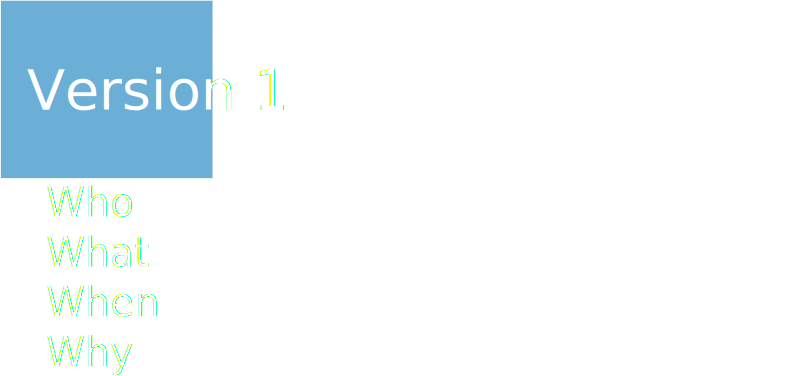
\includegraphics[width=.75\paperwidth]{diagrams/version_control_metadata}}
\end{frame}

\begin{frame}
  \only<1>{\herohigh{\ldots for every version}}%
  \only<2>{\herohigh{git add; git commit}}
  \bottomhalf{\includegraphics[width=.75\paperwidth]{diagrams/version_control_add_commit}}
\end{frame}

\begin{frame}
  \only<1>{\herohigh{Query what changed}}%
  \only<2>{\herohigh{git diff; git log}}
  \bottomhalf{\includegraphics[width=.75\paperwidth]{diagrams/version_control_compare}}
\end{frame}

\begin{frame}
  \only<1>{\herohigh{Undo mistakes}}%
  \only<2>{\herohigh{git revert}}
  \bottomhalf{\includegraphics[width=.75\paperwidth]{diagrams/version_control_revert}}
\end{frame}

\begin{frame}
  \herohigh{Collaboration}%
  \only<1>{\lowerhalf{\large R + {\color{b-purple} git} = nice}}%
  \only<2>{\lowerhalf{\large R + {\color{b-purple} git} + {\color{b-orange}GitHub} = {\color{b-pink}\heart}}}%
  \only<3>{\lowerhalf{\large R + {\color{b-purple} git} + {\color{b-orange}BitBucket} = {\color{b-pink}\heart}}}
\end{frame}

\begin{frame}
  \only<1>{\minionhigh{Work on same code base}}%
  \only<2>{\minionhigh{See what's being changed}}%
  \only<3>{\minionhigh{Who changed it?}}%
  \only<4>{\minionhigh{git blame}}%
  \bottomhalf{%
    \includegraphics<1>[width=.85\paperwidth]{shots/version_control_collaboration}%
    \includegraphics<2>[width=.85\paperwidth]{shots/version_control_changes}%
    \includegraphics<3-4>[width=.85\paperwidth]{shots/version_control_blame}%
    }
\end{frame}

\begin{frame}
  \hero{Version control\\[-.7ex]\color{b-purple} git}
  \lowerhalf{Why doesn't everyone use this all the time?}

  \note{
    \begin{itemize}
    \item The learning curve is difficult.  There are easier tools out
      there, but few with as wide adoption.
    \item Requires discipline.  Easy for newcomers to forget they're
      using it and end up with a commit that just says ``changed
      stuff''.  Like functions, the smaller a change is, the better.
    \item Requires all team members to buy in.
    \item Does not play nicely with binary data (word files), big data
      sets.
    \end{itemize}
  }
\end{frame}

\begin{frame}
  \hero{Version control\\[-.7ex]\color{b-purple} git}
  \lowerhalf{Prospects?}

  \note{
    \begin{itemize}
    \item git is rapidly becoming the main tool for doing version control
      in science.
    \item distinct from \emph{GitHub}, which has become the main
      website that people use to disseminate code, manage
      collaboration.  BitBucket works just as well, even though seems
      less popular among scientists at the moment.  Gitorius and
      self-hosting are less popular still.
    \item alternatives exist: Mercurial is another great VC platform, but
      probably less easy to find people who know it.
    \item The tool shapes the hand -- this tool has changed my habits,
      and those of people I work with, more than any other tool.
    \end{itemize}
  }
\end{frame}

% Make the point that simply docuementing where things come from is
% basically good enough
%
% http://karthik.github.io/useR2014/#data_life_cycle
% http://theconversation.com/the-reinhart-rogoff-error-or-how-not-to-excel-at-economics-13646
% 
\begin{frame}
  \hero{Workflows\\[-.7ex]\color{b-green} make}
  \lowerhalf{It takes a while to make it work}
\end{frame}

\begin{frame}
  \herohigh{Our workflow}
  \bottomhalf{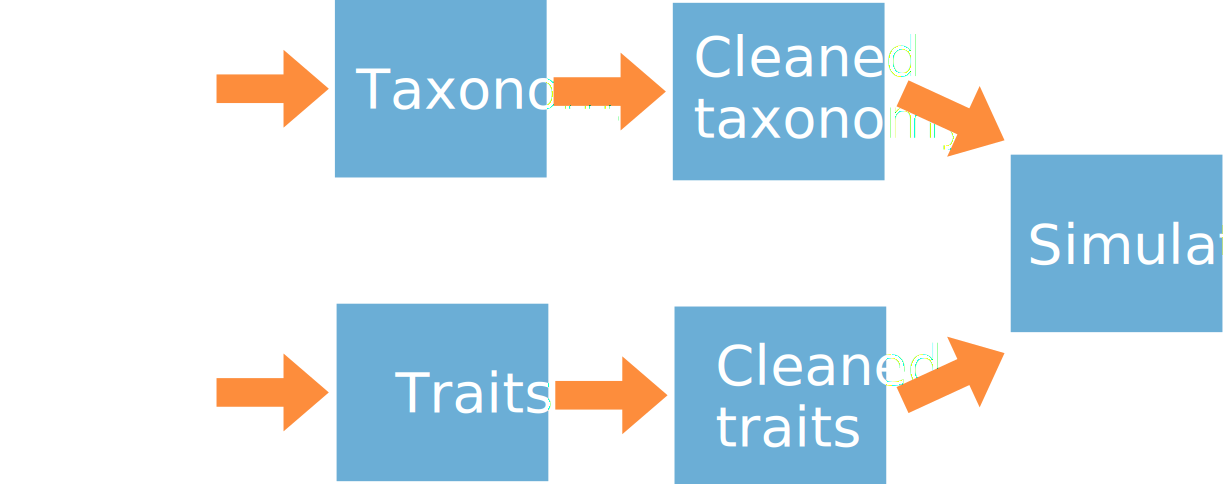
\includegraphics[width=.85\paperwidth]{diagrams/make_workflow}}
  \note{
    Analyses have a chain of dependencies.  Ours was:

    \begin{enumerate}
    \item Download data
    \item Preprocess data to clean it up
    \item Run the simulations
    \end{enumerate}
  }
\end{frame}

\begin{frame}
  \only<1>{\minionhigh{Download data}}
  \only<2>{\minionhigh{Rcurl, API access}}
  \only<3>{\minionhigh{Makefile}}
  \bottomhalf{%
    \includegraphics<3>[height=4ex]{snippets/make_download1}\\[1ex]
    \includegraphics[width=.85\paperwidth]{diagrams/make_workflow_download1}}
\end{frame}

\begin{frame}
  \only<1>{\minionhigh{Process data}}
  \only<2>{\minionhigh{\ldots sausage factory}}
  \only<3>{\minionhigh{Makefile}}
  \bottomhalf{%
    \includegraphics<3>[height=4ex]{snippets/make_process1}\\[1ex]
    \includegraphics[width=.85\paperwidth]{diagrams/make_workflow_process1}}
\end{frame}

\begin{frame}
  \only<1>{\minionhigh{Process data}}
  \only<2>{\minionhigh{\ldots}}
  \only<3>{\minionhigh{Makefile}}
  \bottomhalf{%
    \includegraphics<3>[height=5ex]{snippets/make_simulation}\\[1ex]
    \includegraphics[width=.85\paperwidth]{diagrams/make_workflow_simulation}}
\end{frame}

\begin{frame}
  \hero{Workflows\\[-.7ex]\color{b-green} make}
  \lowerhalf{Why doesn't everyone use this all the time?}
  \note{
    The good:

    \begin{itemize}
    \item we end up with a nice definition of "upstream" sources.
    \item once in place, things run nicely, and have a good chance of
      working elsewhere
    \item a bit of thought helps to separate "inputs" (things that you
      provide) and generated content that you should be able to blow
      away.  This is really important.
    \end{itemize}

    The bad:
    \begin{itemize}
    \item put up a picture of our makefile
    \item Pretty arcane
    \item basically needs replacing with something pleasant, R-ish, and
      enjoyable to use 
    \item knitr's caching can do this to some degree, but I find it fragile.
    \end{itemize}
  }
\end{frame}

\begin{frame}
  \hero{Workflows\\[-.7ex]\color{b-green} make}
  \lowerhalf{Prospects?}
  \note{
    \begin{itemize}
    \item where I hope we can go is a declarative style ``this function
      depends on these things and produces this thing'' that can be used
      to stick together complex analyses.
    \item otherwise I consider this one unsolved for current non-computer
      scientists.
    \end{itemize}
  }
\end{frame}

\begin{frame}
  \hero{Continuous\\[-.7ex]integration\\[-.4ex]\color{b-pink} travis-CI}
  \lowerhalf{Will it work elsewhere?}
  \bottomleft{\href{http://travis-ci.org}{http://travis-ci.org}}
  \note{
    Getting into extra-for-experts territory here

    Basic workflow:

    \begin{enumerate}
    \item Make changes
    \item Check things look OK locally
    \item Push to github
    \item Travis spins up (show a few snippets from the logs)
    \item If there's a problem you get an email (ideally show how this
      works with the link in the email, the changeset, etc).
    \end{enumerate}

    The good:

    I think that this is the future.  If we'd been using this from the
    beginning, we'd have noticed lots of problems that affected us
    later.

    Because you find out as soon as things break, you only have to
    look at a small set of changes.  If you're regularly breaking one
    thing you know where you need to put your time.

    You can collect the output from each run and store them somewhere
    - can turn this into a virtual lab notebook!

    The bad:

    \begin{itemize}
    \item not a perfect fit to research
    \item open source public projects only
    \item not going to work with sensitive data
    \item not going to work with long running jobs
    \item what if your research requires running on a cluster for a month?
    \end{itemize}

    Prospects:

    CI platforms focussed on research probably not far away.
    Several self-hosted solutions that institutions could easily set up
    if there is interest
    \begin{itemize}
    \item Atlassian Bamboo CI (Sydney)
    \item Jenkins
    \item Drone
    \end{itemize}
    Pay for a hosted solution, host on digital ocean, etc.
  }
\end{frame}



\end{document}

%%% Local Variables: 
%%% mode: latex
%%% TeX-PDF-mode: t
%%% TeX-engine: xetex
%%% End: 
